%% SoftwareX article for jaxon --- companion software paper.
%% Built on Elsevier's elsarticle / SoftwareX OSP template.
\documentclass[preprint,12pt,a4paper]{elsarticle}

\usepackage{amssymb}
\usepackage{amsmath}
\usepackage{hyperref}
\usepackage{xurl}   % allow long URLs to break anywhere (keeps them inside table cells)
\usepackage{xcolor}
\setlength{\parindent}{0pt}

\journal{SoftwareX}

\begin{document}
\renewcommand{\labelenumii}{\arabic{enumi}.\arabic{enumii}}

\begin{frontmatter}

\title{jaxon: a differentiable, GPU-native simulator for peripheral-nerve fiber models}

\author[meduni]{David Lung}
\author[meduni,lbi]{Max Haberbusch\corref{cor1}}
\ead{max.haberbusch@meduniwien.ac.at}
\cortext[cor1]{Corresponding author.}

\address[meduni]{Center for Medical Physics and Biomedical Engineering, Medical University of Vienna, Vienna, Austria}
\address[lbi]{Ludwig Boltzmann Institute for Cardiovascular Research, Vienna, Austria}

\begin{abstract}
\emph{jaxon} is an open-source, fully differentiable and GPU-native reimplementation of the
canonical peripheral-nerve fiber models in JAX/Jaxley: the myelinated
McIntyre--Richardson--Grill (MRG) and Sweeney axons and the unmyelinated Sundt and Rattay
C-fibers. It reproduces NEURON's \texttt{extracellular} mechanism through a custom
backward-Euler coupled intracellular/periaxonal double-cable solver, agreeing with
pyfibers-wrapped NEURON on $99.6\,\%$ of $943$ activation-threshold configurations within
$1\,\%$ and matching conduction velocity to machine precision. Because the entire forward
model is expressed in JAX, it is both vectorized---simulating whole fiber populations in
parallel and reaching a geometric-mean ${\sim}820\times$ speedup at $N=100{,}000$ fibers on
a single GPU---and differentiable, so extracellular-stimulation parameters (per-contact
amplitudes, waveform shape, and electrode position) can be optimized directly through the
cable equation rather than grid-searched. \emph{jaxon} slots into existing peripheral-nerve
modeling pipelines as a gradient-enabled, population-scale replacement for the NEURON
forward solver.
\end{abstract}

\begin{keyword}
peripheral nerve stimulation \sep fiber model \sep differentiable simulation \sep JAX \sep
GPU \sep neuromodulation \sep selectivity optimization
\end{keyword}

\end{frontmatter}

%\linenumbers

\section*{Required Metadata}

\section*{Current code version}

\begin{table}[!h]
\begin{tabular}{|l|p{6.0cm}|p{6.0cm}|}
\hline
\textbf{Nr.} & \textbf{Code metadata description} & \textbf{Please fill in this column} \\
\hline
C1 & Current code version & v1.0.0 \\
\hline
C2 & Permanent GitHub link to code/repository used for this code version & \url{https://github.com/CellularSyntax/jaxon} \\
\hline
C3 & Legal Code License   & MIT \\
\hline
C4 & Code versioning system used & git \\
\hline
C5 & Software code languages, tools, and services used & Python 3.11; JAX 0.6.2, Jaxley 0.13.0, Optax 0.2.8, NumPy 2.2.6, SciPy 1.15.3, Matplotlib 3.10.9; NEURON 9.0.1 and PyFibers 0.8.5 (reference/validation only); optional CUDA 12 for GPU execution \\
\hline
C6 & Compilation requirements, operating environments \& dependencies & Platform-independent (Linux/macOS/Windows-WSL2); a Conda environment (\texttt{environment.yml}) provides all dependencies; an optional NVIDIA GPU (CUDA 12) enables batched GPU execution \\
\hline
C7 & If available, link to developer documentation/manual & \url{https://github.com/CellularSyntax/jaxon} (README, REPRODUCE.md, AUDIT.md) \\
\hline
C8 & Support email for questions & \nolinkurl{max.haberbusch@meduniwien.ac.at} \\
\hline
\end{tabular}
\caption{Code metadata.}
\label{tab:meta}
\end{table}

\section{Motivation and significance}

Electrical stimulation of peripheral nerves is an established therapy for a growing range of
conditions, and selecting where to place an electrode and how to shape the stimulus
increasingly relies on computational models. The standard modeling approach couples a
volume-conductor description of the tissue---typically solved by the finite-element method
(FEM)---to biophysical, multi-compartment cable models of individual
axons~\cite{mcneal,mcintyre}. The extracellular potential computed along each fiber drives
the membrane model, and threshold and recruitment follow. The reference implementation of
the fiber side of this pipeline is NEURON~\cite{neuron}, most conveniently accessed through
PyFibers~\cite{pyfibers}, which wraps the canonical published axon models.

This reference stack is accurate but has two structural limitations for modern
neural-interface design. First, it is \emph{serial}: NEURON simulates one fiber at a time on
the CPU, so scoring an optimized stimulus over an entire fiber population---hundreds to tens
of thousands of axons per nerve---is prohibitively slow. To stay tractable, models almost
universally reduce each fascicle to one or a few representative fibers, and whether that
reduction biases the selectivity they predict has been effectively untestable. Second, it is
\emph{non-differentiable}: because there is no gradient of the fiber response with respect to
the stimulus, stimulation parameters must be tuned by grid search or gradient-free
optimization, both of which scale poorly as the number of contacts and waveform degrees of
freedom grows. GPU-accelerated surrogates such as AxonML~\cite{axonml} address the speed
problem by learning a fast approximation of the threshold, but a surrogate is a fit to the
biophysics rather than the biophysics itself.

\emph{jaxon} was built to remove both limitations while keeping the biophysics exact. It
reimplements the canonical peripheral-nerve fiber models---the myelinated MRG~\cite{mcintyre}
and Sweeney~\cite{sweeney} axons and the unmyelinated Sundt~\cite{sundt} and
Rattay~\cite{rattay} C-fibers---in JAX~\cite{jax} on top of the Jaxley differentiable cable
simulator~\cite{jaxley}, and adds a custom backward-Euler solver for the coupled
intracellular/periaxonal double-cable equation that is the principled equivalent of NEURON's
\texttt{extracellular} mechanism. Because the whole forward model is JAX, it is
simultaneously \emph{vectorized}---running whole populations in parallel with
\texttt{jax.vmap}---and \emph{differentiable}---exposing exact gradients of the fiber response
with respect to the stimulus. \emph{jaxon} is validated against pyfibers-wrapped NEURON and
reaches a geometric-mean ${\sim}820\times$ speedup at $N=100{,}000$ fibers on one GPU, fast
enough to optimize and then re-score whole-nerve populations. A companion
paper~\cite{companion} uses \emph{jaxon} to show that the common single-representative-fiber
reduction overestimates deliverable selectivity in a species-dependent way; the present paper
describes the software itself.

\section{Software description}

\subsection{Software architecture}

\emph{jaxon} is organized as a differentiable forward model wrapped by an optimization and
analysis layer (Fig.~\ref{fig:arch}). At its center is a vectorized integrator of the coupled
$(V_i, V_{px})$ cable equation that maps a set of per-contact stimulus amplitudes (and,
optionally, waveforms and electrode positions) onto the membrane response of an arbitrary
number of fibers at once. The model is used through three interchangeable entry points that
all act on the same underlying functions: a Python package (\texttt{jaxfibers}) for library
use, a set of experiment scripts (\texttt{experiments\_v2}) that reproduce the paper, and
SLURM batch drivers for cluster runs.

The package is structured by concern:
\begin{itemize}
  \item \texttt{jaxfibers.channels} --- each NMODL ion-channel mechanism hand-translated into
        a pure-JAX \texttt{Channel} class, with rate constants checked against the published
        \texttt{.mod} formulas to machine precision;
  \item \texttt{jaxfibers.fibers} --- morphology builders, one per model, returning a
        \texttt{jaxley.Cell} and a geometry dataclass describing the per-compartment static
        parameters;
  \item \texttt{jaxfibers.stim} --- the intracellular and point-source extracellular stimulus
        helpers, the coupled backward-Euler solver
        (\texttt{extracellular\_coupled.py}), the vmapped multi-fiber forward pass
        (\texttt{batch\_solve.py}), and the multi-contact ring-cuff field;
  \item \texttt{jaxfibers.optim} --- the recruitment/activation proxy, the selectivity index,
        and the Adam optimization loops.
\end{itemize}

The coupled solver integrates the double-cable equation by backward Euler; each time step is a
$2\times2$ block-tridiagonal system in the interleaved intracellular and periaxonal unknowns
(Fig.~\ref{fig:solver}),
solved directly by a JAX-compatible block-Thomas sweep (verified to
$5.6\times10^{-11}$~mV against a dense LU reference), with back-substitution via
\texttt{jax.lax.associative\_scan} for $O(\log n)$ depth.
\begin{figure}[htbp]
\centering
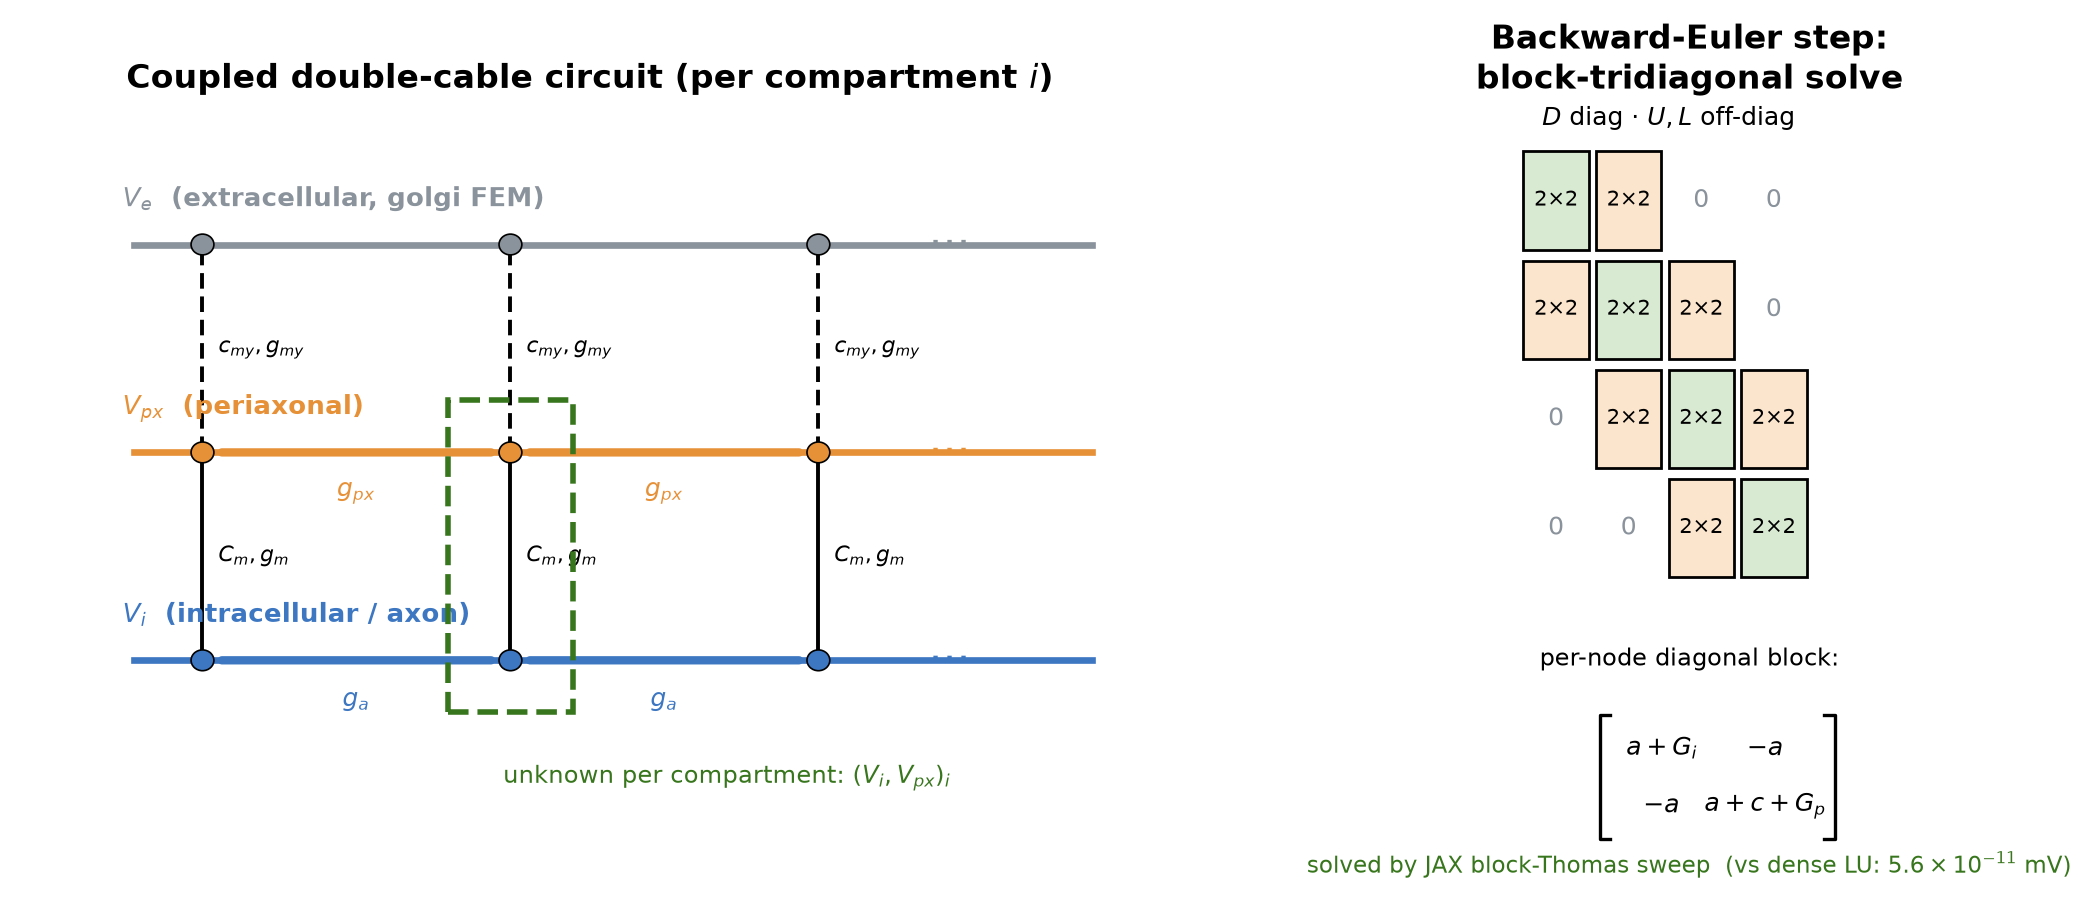
\includegraphics[width=\linewidth]{figures/jaxon_solver.png}
\caption{The coupled solver. Left: the double-cable circuit \emph{jaxon} integrates---each
compartment couples an intracellular node ($V_i$), a periaxonal space ($V_{px}$), and the
externally imposed extracellular potential ($V_e$, supplied by \emph{golgi} FEM lead fields),
through the axolemmal ($C_m, g_m$) and myelin ($c_{my}, g_{my}$) admittances and the axial
conductances ($g_a$, $g_{px}$). Right: each backward-Euler step is a block-tridiagonal system in
the interleaved $(V_i, V_{px})$ unknowns, whose $2\times2$ diagonal blocks are solved directly by
a JAX-compatible block-Thomas sweep (verified to $5.6\times10^{-11}$~mV against a dense LU
reference).}
\label{fig:solver}
\end{figure}
 Because every operation is a JAX
primitive, the same forward pass is (i) batched over fibers with \texttt{jax.vmap} for
population-scale throughput and (ii) differentiated with reverse-mode autodiff (or a packed
finite-difference gradient) for stimulus optimization. For the cohort application, per-contact
lead fields are supplied by the \emph{golgi} platform~\cite{golgi_platform,golgi_software} from
histology-segmented nerve geometries; a lightweight analytic point-source field is included for
local demonstrations.

\begin{figure}[!h]
\centering
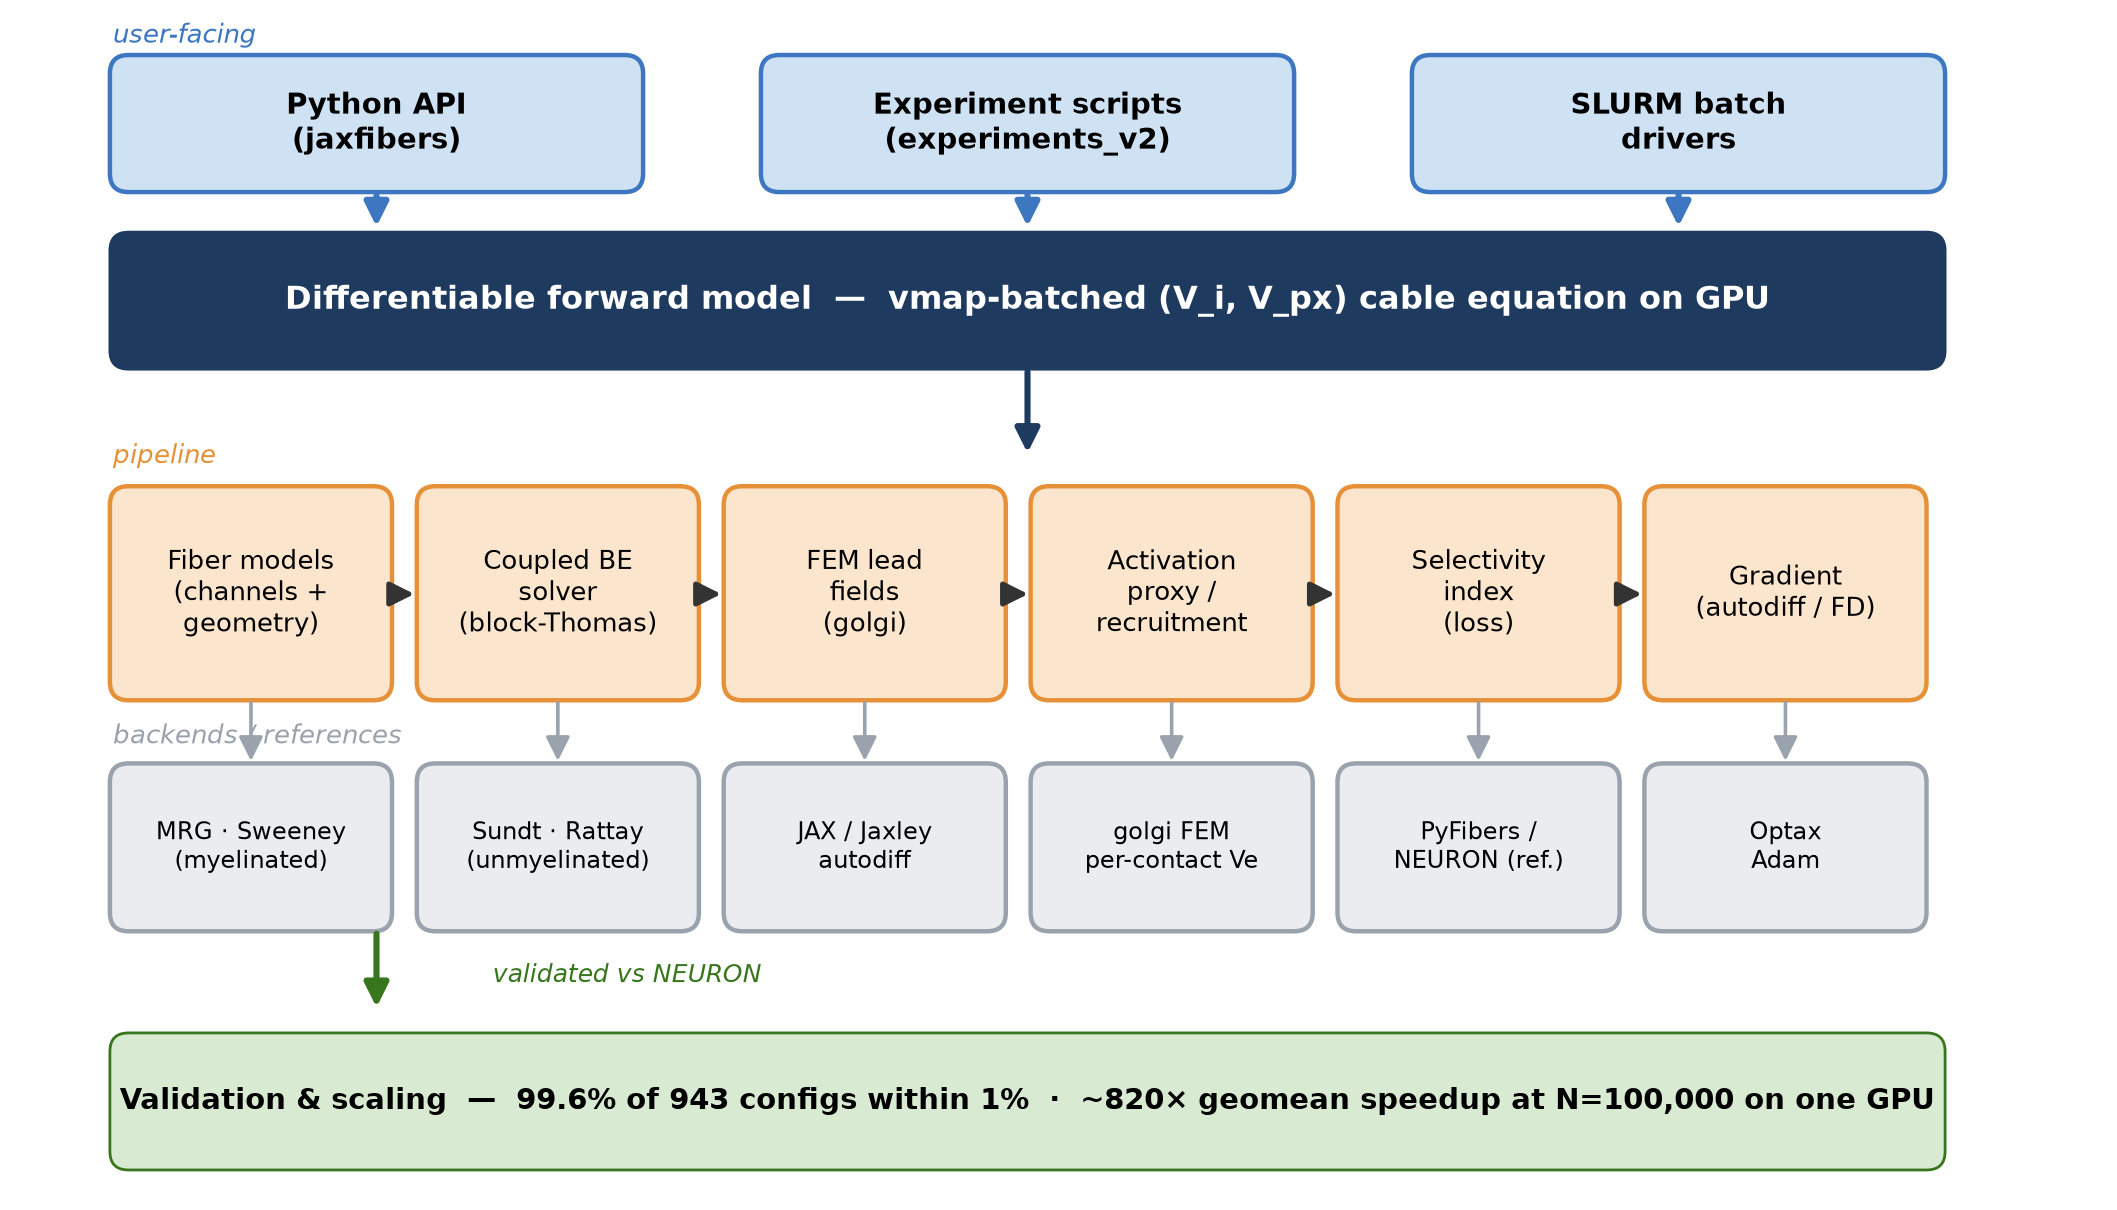
\includegraphics[width=\linewidth]{figures/jaxon_architecture.png}
\caption{Architecture of \emph{jaxon}. Three user-facing entry points (the \texttt{jaxfibers}
Python package, the \texttt{experiments\_v2} scripts, and SLURM batch drivers) share one
differentiable, \texttt{vmap}-batched forward model of the coupled $(V_i, V_{px})$ cable
equation. The pipeline runs on JAX/Jaxley (autodiff), \emph{golgi} FEM per-contact lead fields,
and PyFibers/NEURON as the validation reference; the myelinated (MRG, Sweeney) and unmyelinated
(Sundt, Rattay) fiber models, the block-Thomas coupled solver, the activation/selectivity
losses, and the gradient form the stages. The whole model is validated against NEURON and
scales to $N=100{,}000$ fibers on one GPU.}
\label{fig:arch}
\end{figure}

\begin{figure}[htbp]
\centering
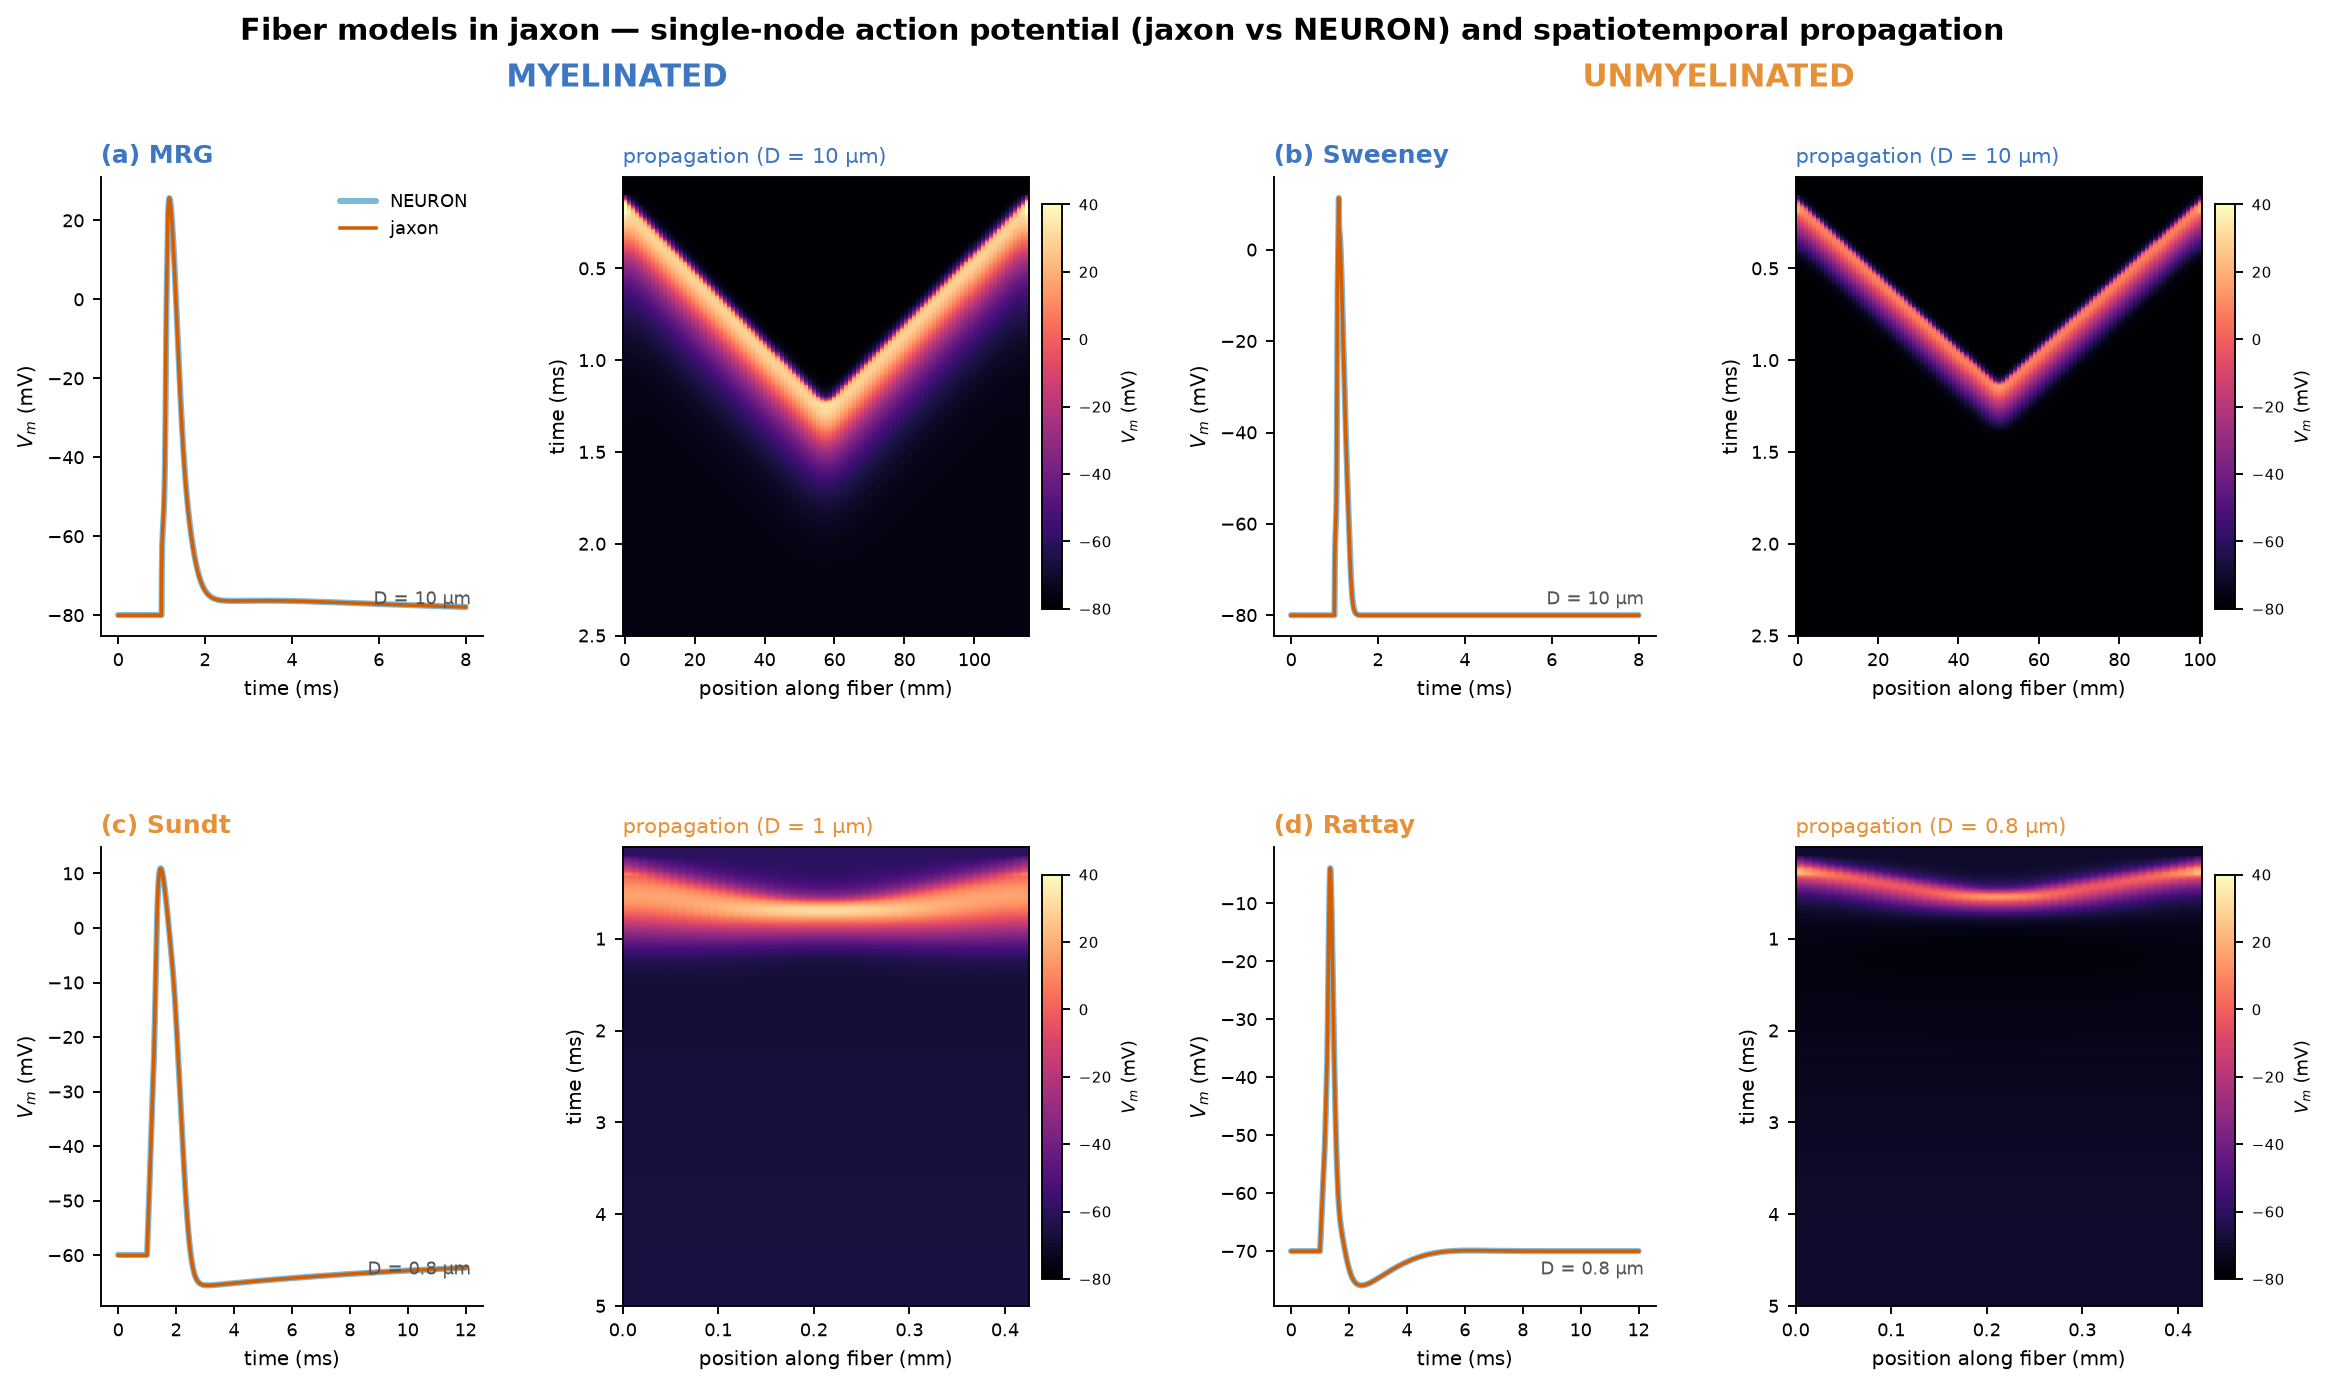
\includegraphics[width=\linewidth]{figures/jaxon_models.png}
\caption{The four fiber models integrated in \emph{jaxon}, grouped by class. For each model,
left: the single-node membrane action potential, with \emph{jaxon} (orange) overlaid on the
pyfibers-wrapped NEURON reference (blue); right: the spatiotemporal $V_m(\text{position},
\text{time})$ propagation. The myelinated MRG and Sweeney axons (a, b) show fast saltatory
propagation---here two counter-propagating spikes meeting and annihilating in a characteristic
collision---while the unmyelinated Sundt and Rattay C-fibers (c, d) propagate slowly and
continuously. All curves are \emph{jaxon} output; the NEURON overlay is the validation reference.}
\label{fig:models}
\end{figure}

\subsection{Software functionalities}
\label{sec:func}

\emph{jaxon}'s major functionalities are:

\begin{enumerate}
  \item \textbf{Canonical fiber models.} Four published axon models---myelinated
        MRG~\cite{mcintyre} (with both the original and interpolated parameter tables) and
        Sweeney~\cite{sweeney}, and unmyelinated Sundt~\cite{sundt} and Rattay~\cite{rattay}
        C-fibers---reimplemented as pure-JAX channels and morphologies
        (Fig.~\ref{fig:models}).
  \item \textbf{Coupled extracellular solver.} A backward-Euler integrator for the two-state
        $(V_i, V_{px})$ double-cable equation---the principled equivalent of NEURON's
        \texttt{extracellular} mechanism rather than the single-cable activating-function
        approximation---solved by a JAX-compatible $2\times2$ block-Thomas sweep.
  \item \textbf{Population-scale batched forward pass.} \texttt{jax.vmap} packs $N$ fibers into
        a single vectorized simulation, enabling whole-nerve populations to be simulated and
        re-scored on one GPU.
  \item \textbf{Differentiable stimulus optimization.} Three optimization modes: per-contact
        rectangular amplitudes via a packed finite-difference gradient ($K{+}1$ configurations
        in one forward pass); arbitrary $K\times T$ waveforms via reverse-mode autodiff through
        the ODE scan (with gradient checkpointing); and joint amplitude-plus-electrode-position
        search, with the extracellular field recomputed differentiably each step.
  \item \textbf{Selectivity scoring.} A recruitment (activation) proxy and a selectivity index
        defined as the difference between the recruited fraction of on-target and off-target
        fibers, usable both as an optimization objective and as a post-hoc population score.
  \item \textbf{FEM-field and multi-contact support.} Per-contact lead fields from the
        \emph{golgi} platform over histology-segmented nerves and a multi-contact ring cuff,
        with a superposition-based current-steering model; an analytic point-source field is
        provided for demonstrations and tests.
  \item \textbf{Validation and benchmarking.} Scripts that reproduce the threshold,
        conduction-velocity, and propagation-phenomena comparisons against pyfibers-wrapped
        NEURON, and the CPU/GPU scaling benchmark.
\end{enumerate}

\subsection{Sample code}

The library exposes the model-building, forward-solve, loss, and optimization functions
directly, so a study is assembled from a few calls: build one or more fibers with
\texttt{jaxfibers.fibers} (returning a Jaxley \texttt{Cell} and a geometry dataclass); assemble
the per-fiber static parameters and initial states with \texttt{stack\_fiber\_statics} /
\texttt{initial\_states\_batch}; run the batched coupled solve with \texttt{batch\_integrate\_m\_max};
and score or optimize with \texttt{jaxfibers.optim} (\texttt{selectivity\_index},
\texttt{run\_rect\_optimization}). Section~\ref{sec:examples} gives three worked, runnable
examples following this progression.

\section{Illustrative examples}
\label{sec:examples}

The three examples below show the typical usage progression---validating one fiber against
NEURON, simulating a population in a single batched pass, and optimizing a multi-contact stimulus
by differentiating through that pass. All are runnable from the released package; the
corresponding end-to-end scripts live in \texttt{experiments\_v2/}.

\paragraph{Example 1 --- build a fiber and compute an activation threshold.}
A single model fiber is built, placed in an extracellular field, and its activation threshold is
obtained by the same bisection used for the NEURON comparison. This is the unit that the
validation suite runs across $943$ configurations.

{\footnotesize
\begin{verbatim}
import numpy as np
from jaxfibers.fibers import mrg
from jaxfibers.stim.batch_solve import (build_fiber_statics,
                                        initial_states_batch,
                                        batch_integrate_m_max)
from jaxfibers.stim.extracellular import (point_source_potentials_mV,
                                          rectangular_waveform)

dt = 0.005                              # ms

# Build an MRG fiber (Jaxley Cell + geometry metadata).
cell, geom = mrg.build_mrg(diameter=10.0, temperature=37.0)

# Static point-source profile (unit current) 1 mm above the fiber,
# times a rectangular pulse -> the [T, n_comp] extracellular sequence.
t_grid = np.arange(0.0, 2.0, dt)
profile = point_source_potentials_mV(mrg.section_centers_um(geom),
                                     src_y_um=1000.0, i0_mA=-1.0)   # mV per mA
wave    = rectangular_waveform(t_grid, delay_ms=0.1, pw_ms=0.1, amp=0.5)  # mA
Ve_seq  = wave[:, None] * profile[None, :]        # [T, n_comp]

# Integrate the coupled (V_i, V_px) cable equation; batch_integrate_m_max
# returns the peak Na m-gate, the proxy jaxon uses to decide firing.
fs = build_fiber_statics(geom, dt=dt)
s0 = initial_states_batch([geom])
# ... scale `amp` by bisection until the fiber just fires -> threshold.
\end{verbatim}
}

\paragraph{Example 2 --- simulate a whole population in one batched pass.}
The same forward model, stacked over $N$ fibers with \texttt{jax.vmap}, simulates an entire
population in a single call. This is the operation that runs at a geometric-mean
${\sim}820\times$ speedup over serial NEURON at $N=100{,}000$ fibers, and that makes
population-scale re-scoring cheap.

{\footnotesize
\begin{verbatim}
from jaxfibers.stim.batch_solve import (stack_fiber_statics,
                                        initial_states_batch,
                                        batch_integrate_m_max)
from jaxfibers.optim.losses import activation_proxy_batch, selectivity_index

# A population of fibers seeded across the nerve cross-section.
geoms = [mrg.build_mrg(diameter=5.7)[1] for _ in range(n_fibers)]
node_idx = [mrg.node_indices(g) for g in geoms]

fs_batch = stack_fiber_statics(geoms, dt=dt)       # [n_fibers, n_comp, ...]
s0_batch = initial_states_batch(geoms)

# Ve_seq_batch: [n_fibers, T, n_comp] -- per-fiber extracellular sequence,
# here from the golgi FEM per-contact lead fields under a chosen stimulus.
m_max = batch_integrate_m_max(fs_batch, s0_batch, Ve_seq_batch, dt=dt)

# Recruitment per fiber, then the population selectivity index.
acts = activation_proxy_batch(m_max, node_idx)
si   = selectivity_index(acts, target_mask)        # SI in [-1, 1]
\end{verbatim}
}

\paragraph{Example 3 --- optimize a multi-contact stimulus by gradient descent.}
Because the batched forward pass is differentiable, the per-contact amplitudes of a cuff are
optimized directly against the selectivity objective. \texttt{run\_rect\_optimization} drives an
Adam loop through the exact cable solve, using the packed finite-difference gradient
($K{+}1$ configurations per forward pass); an autodiff variant
(\texttt{run\_rect\_optimization\_autodiff}) differentiates through the ODE scan for arbitrary
waveforms.

{\footnotesize
\begin{verbatim}
from jaxfibers.optim.optimizer import run_rect_optimization

# Ve_unit: [K, n_fibers, n_comp] -- unit lead field of each of the K contacts.
# pulse_mask: [T] -- the rectangular time course shared by all contacts.
amps, history = run_rect_optimization(
    fs_batch, s0_batch, Ve_unit, pulse_mask,
    node_indices=node_idx, target_mask=target_mask,
    dt=dt, n_steps=90, lr=8e-2,
    amp_clip=(-2.5, 2.5),          # per-contact amplitude bounds (mA)
)

# Re-score the optimized stimulus on the FULL population (cheap in jaxon):
Ve_opt = jnp.einsum("k,knc->nc", amps, Ve_unit)[:, None, :] * pulse_mask[None, :, None]
m_max  = batch_integrate_m_max(fs_batch, s0_batch, Ve_opt, dt=dt)
print("population SI:", selectivity_index(activation_proxy_batch(m_max, node_idx),
                                          target_mask))
\end{verbatim}
}

All three examples are reproducible from the released code; \texttt{REPRODUCE.md} documents the
full path from a fiber build to every figure and reported number in the companion
study~\cite{companion}.

\section{Impact}

\emph{jaxon} changes what is computationally feasible in peripheral-nerve-stimulation modeling
along two axes that the reference NEURON stack leaves closed.

First, it \textbf{makes population-scale fiber modeling routine}. By expressing the canonical
axon models as a \texttt{vmap}-batched JAX forward pass, \emph{jaxon} simulates whole fiber
populations on a single GPU at a geometric-mean ${\sim}820\times$ speedup over serial NEURON,
turning a previously prohibitive whole-nerve re-scoring into a step cheap enough to run inside
an optimization loop. This directly enables the central question of the companion
study~\cite{companion}---whether reducing each fascicle to a representative fiber biases predicted
selectivity---which was untestable precisely because the population simulation was too expensive.

Second, it \textbf{makes the stimulus itself an optimization variable}. Because the whole model
is differentiable, per-contact amplitudes, arbitrary waveforms, and electrode positions can be
optimized by gradient descent through the exact cable equation, rather than by grid search or a
learned surrogate. Unlike a surrogate model, the gradient is of the biophysics, not of a fit to
it, so an optimized stimulus can be validated in the same tool that produced it.

Third, it \textbf{drops into existing pipelines with minimal friction}. \emph{jaxon} is
validated against the community-standard PyFibers/NEURON reference ($99.6\,\%$ of $943$
configurations within $1\,\%$; conduction velocity to machine precision) and released
open-source under a permissive license, so it can serve as a gradient-enabled, population-scale
replacement for the NEURON forward solver wherever fiber-level thresholds are needed. Its
per-contact-lead-field interface connects it to FEM tooling such as \emph{golgi}, positioning it
as an interoperable component rather than a standalone silo.

By combining exact, validated biophysics with GPU-scale throughput and end-to-end
differentiability, \emph{jaxon} lets neural-interface researchers ask and answer optimization and
population-scale questions that the established serial, non-differentiable tools cannot.

\section{Conclusions}

\emph{jaxon} is an open-source, differentiable, GPU-native reimplementation of the canonical
peripheral-nerve fiber models---MRG and Sweeney (myelinated) and Sundt and Rattay
(unmyelinated)---built on JAX/Jaxley with a custom coupled $(V_i, V_{px})$ backward-Euler solver.
It matches pyfibers-wrapped NEURON on $99.6\,\%$ of $943$ threshold configurations and to machine
precision in conduction velocity, scales to a geometric-mean ${\sim}820\times$ speedup at
$N=100{,}000$ fibers on one GPU, and exposes exact gradients of the fiber response for
stimulus optimization. Validated against NEURON and applied to a species-dependent selectivity
question in the companion paper~\cite{companion}, \emph{jaxon} provides a gradient-enabled,
population-scale replacement for the NEURON forward solver in peripheral-nerve modeling
pipelines.

\section*{Data availability and licensing}

\emph{jaxon} is released as open-source software under the MIT license (code metadata C3/S3).
The source code is available on GitHub (\url{https://github.com/CellularSyntax/jaxon}), and the
tagged v1.0.0 release is archived on Zenodo~\cite{zenodo_jaxon_code}. The processed data required
to reproduce every figure and reported number---the \emph{golgi}-derived per-contact lead fields
and the validation, scaling, and cohort-sweep outputs---is archived as a companion Zenodo data
record~\cite{zenodo_jaxon_data} under the Creative Commons Attribution 4.0 International
(CC-BY-4.0) license, distinct from the software license. The raw finite-element meshes are
\emph{golgi} outputs and are available through the \emph{golgi} platform~\cite{golgi_platform,golgi_software}
and the underlying SPARC datasets. Reproduction is documented in \texttt{REPRODUCE.md} in the
repository.

\section*{CRediT authorship contribution statement}
\textbf{David Lung:} Software, Investigation, Validation, Writing -- review \& editing.
\textbf{Max Haberbusch:} Conceptualization, Methodology, Software, Supervision, Funding
acquisition, Writing -- original draft, Writing -- review \& editing.

\section*{Acknowledgements}

The authors thank the Medical University of Vienna for access to high-performance computing
resources. \emph{(Funding acknowledgements to be completed by the authors.)}

\begin{thebibliography}{00}

\bibitem{companion} D. Lung, M. Haberbusch, A GPU-native, differentiable fiber simulator reveals
a species-dependent selectivity penalty in reduced-order peripheral-nerve models, companion
manuscript (under review).

\bibitem{mcneal} D.R. McNeal, Analysis of a model for excitation of myelinated nerve, IEEE
Transactions on Biomedical Engineering 23 (1976) 329--337.

\bibitem{mcintyre} C.C. McIntyre, A.G. Richardson, W.M. Grill, Modeling the excitability of
mammalian nerve fibers: influence of afterpotentials on the recovery cycle, Journal of
Neurophysiology 87 (2002) 995--1006.

\bibitem{sweeney} J.D. Sweeney, J.T. Mortimer, D. Durand, Modeling of mammalian myelinated nerve
for functional neuromuscular stimulation, in: IEEE 9th Annual Conference of the Engineering in
Medicine and Biology Society, 1987, pp.\ 1577--1578.

\bibitem{sundt} D. Sundt, N. Gamper, D.B. Jaffe, Spike propagation through the dorsal root
ganglia in an unmyelinated sensory neuron: a modeling study, Journal of Neurophysiology 114
(2015) 3140--3153.

\bibitem{rattay} F. Rattay, Analysis of models for extracellular fiber stimulation, IEEE
Transactions on Biomedical Engineering 36 (1989) 676--682.

\bibitem{neuron} M.L. Hines, N.T. Carnevale, The NEURON simulation environment, Neural
Computation 9 (1997) 1179--1209.

\bibitem{pyfibers} D.P. Marshall, et al., PyFibers: an open-source NEURON-Python package to
simulate responses of model nerve fibers to electrical stimulation, PLOS Computational Biology
21 (12) (2025) e1013764.

\bibitem{jax} J. Bradbury, et al., JAX: composable transformations of Python+NumPy programs,
2018. \url{http://github.com/jax-ml/jax}.

\bibitem{jaxley} M. Deistler, et al., Differentiable simulation enables large-scale training of
detailed biophysical models of neural dynamics, 2024.

\bibitem{axonml} M.A. Hussain, W.M. Grill, N.A. Pelot, Highly efficient modeling and
optimization of neural fiber responses to electrical stimulation, Nature Communications 15
(2024) 7597.

\bibitem{golgi_platform} D. Lung, Y. Jia, R. Blumer, L. Reissig, L.M. Zopf, P. Heimel, C. Kraus,
A. Moro, M. Fachino, M. Haberbusch, golgi: an open-source graphical platform for
image-to-recruitment modeling of peripheral nerve stimulation, bioRxiv 2026.07.10.737529.
\url{https://doi.org/10.64898/2026.07.10.737529}.

\bibitem{golgi_software} D. Lung, Y. Jia, A. Moro, M. Fachino, M. Haberbusch, golgi: open-source
software for automated nerve model generation and recruitment simulation, bioRxiv
2026.07.10.737846. \url{https://doi.org/10.64898/2026.07.10.737846}.

\bibitem{zenodo_jaxon_code} D. Lung, M. Haberbusch, jaxon: a differentiable, GPU-native simulator
for peripheral-nerve fiber models (v1.0.0) [software], Zenodo, 2026.
\url{https://doi.org/10.5281/zenodo.XXXXXXX}.

\bibitem{zenodo_jaxon_data} D. Lung, M. Haberbusch, Reproduction data archive for jaxon [dataset],
Zenodo, 2026. \url{https://doi.org/10.5281/zenodo.YYYYYYY}.

\end{thebibliography}

\section*{Current executable software version}

\begin{table}[!h]
\begin{tabular}{|l|p{6.0cm}|p{6.0cm}|}
\hline
\textbf{Nr.} & \textbf{(Executable) software metadata description} & \textbf{Please fill in this column} \\
\hline
S1 & Current software version & v1.0.0 \\
\hline
S2 & Permanent link to executables of this version & Zenodo, \url{https://doi.org/10.5281/zenodo.XXXXXXX} (v1.0.0) \\
\hline
S3 & Legal Software License & MIT (matches C3) \\
\hline
S4 & Computing platforms/Operating Systems & Linux, macOS, Windows (WSL2) \\
\hline
S5 & Installation requirements \& dependencies & Conda environment (\texttt{environment.yml}); JAX 0.6.2, Jaxley 0.13.0, Optax; NEURON 9.0.1 + PyFibers 0.8.5 for the validation reference; optional NVIDIA GPU + CUDA 12 for batched GPU execution \\
\hline
S6 & If available, link to user manual & \url{https://github.com/CellularSyntax/jaxon} \\
\hline
S7 & Support email for questions & \nolinkurl{max.haberbusch@meduniwien.ac.at} \\
\hline
\end{tabular}
\caption{Software metadata.}
\label{tab:exec}
\end{table}

\end{document}
